\chapter{Diseño y Desarrollo de la plataforma}
\label{chap:diseno_desarrollo}

En este capítulo se explicará todo el proceso de diseño y desarrollo de la plataforma, dando especial énfasis a la justificación de las decisiones tomadas y a la explicación de los distintos problemas que se han ido encontrando a lo largo del proceso. En concreto, se detallará el diseño de la base de datos, el desarrollo del \textit{backend} y el desarrollo del \textit{frontend}. No obstante, antes de entrar en detalle en cada una de estas secciones, se explicará el proceso inicial de desarrollo de la plataforma y se justificarán las tecnologías elegidas, cumplimentando así la sección \ref{sec:arquitectura_sistema} del capítulo \ref{chap:marco_teorico}.

% \textcolor{red}{Explicar que s'ha decidit fer un saas i una app web degut a les aventatges anteriorment esmentades.}

% \textcolor{red}{Ja s'ha dit que es farà servir React i Django i s'ha explicat breument com funcionen. Afegir el perquè d'aquestes eleccions.}

\section{Proceso inicial de desarrollo de la plataforma}
\label{sec:proceso_desarrollo}

El desarrollo de la aplicación web no surge de simplemente decidir qué tecnologías se van a utilizar y empezar a programar. Antes de comenzar a desarrollar la plataforma se ha llevado a cabo un proceso de diseño que ha permitido definir la arquitectura del sistema, las tecnologías a utilizar y el flujo de trabajo.

\subsection{Separación de tecnologías \textit{frontend} y \textit{backend}}

El primer paso que se ha realizado y una vez ya definido el objetivo de la aplicación y las funcionalidades que se querían implementar, se ha llevado a cabo un análisis de como estructurar la plataforma. Como ya se ha comentado en la sección \ref{sec:arquitectura_sistema}, se ha optado por una arquitectura dividida en dos partes: el \textit{backend}, incluyendo la base de datos, y el \textit{frontend}. No obstante, a pesar de que Django ofrece la posibilidad de crear ambas partes, se ha decidido utilizar React. Esta decisión ha supuesto un reto, ya que ha significado realizar un \textit{frontend} entero además de preparar una API en el \textit{backend} para que ambos se puedan comunicar. Sin embargo, esta decisión ha permitido crear una aplicación más escalable, flexible y, sobre todo, dinámica.

Django es un \textit{framework} que funciona del lado del servidor, lo que significa que cada vez que se quiere mostrar una página distinta, el servidor tiene que procesar la petición y devolver la página completa. De esta manera, cuando el usuario cambia de página, el servidor carga todos los recursos (HTML, CSS y JavaScript) y los rellena con los datos necesarios, sirviendo una página estática. Por el contrario, React es un \textit{framework} que funciona del lado del cliente, lo que significa que el servidor solo tiene que enviar los datos necesarios y el cliente se encarga de mostrar la información. Con esto, el servidor solo tiene que enviar los datos necesarios y el cliente se encarga de mostrar la información. Esto permite crear aplicaciones más dinámicas y rápidas, ya que no es necesario recargar la página cada vez que se quiere mostrar un nuevo contenido.

Este enfoque, a pesar de ser más complejo, es el estándar en la actualidad y es por este motivo que se ha optado por esta división de tecnologías.

\section{Diseño de la base de datos}
\label{sec:diseno_base_datos}

Para estructurar el proyecto, se ha optado por empezar definiendo la base de datos. Diseñar la base de datos inicialmente permite tener una visión general de como se va a estructurar el proyecto y como sus distintas partes se van a relacionar entre sí. Al fin y al cabo, la base de datos es el núcleo de la aplicación, ya que de ella dependen todas las funcionalidades.

\subsection{Bloques de funcionalidades}

Antes de empezar a diseñar la base de datos, se deben definir las funcionalidades claves de la aplicación para así poder estructurar los datos de manera que se puedan implementar de la mejor manera posible. En este caso, las funcionalidades claves son las siguientes:

\begin{itemize}
    \item \textbf{Gestión de pedidos:} La herramienta debe centralizar todos los pedidos de los distintos canales de venta en línea y permitir la gestión de los mismos. Esto incluye la posibilidad de crear, editar y eliminar pedidos, así como la posibilidad de marcar un pedido como enviado o entregado.
    \item \textbf{Gestión de productos:} La herramienta debe permitir la gestión de los productos disponibles en los distintos canales de venta en línea. Esto incluye la posibilidad de crear, editar y eliminar productos de los distintos canales, así como la posibilidad de editar sus atributos, tales como el precio, la descripción y la imagen, entre muchos otros.
    \item \textbf{Gestión de canales:} La herramienta debe permitir la gestión de los distintos canales de venta en línea. Esto incluye la posibilidad de crear, editar y eliminar canales.
    \item \textbf{Gestión de usuarios:} La herramienta debe permitir la gestión de los usuarios que pueden acceder a la aplicación. Esto incluye la posibilidad de crear, editar y eliminar usuarios, así como la posibilidad de asignarles distintos permisos y roles dentro de la aplicación.
\end{itemize}

Con las tres funcionalidades clave definidas, se puede concluir que la base de datos debe contener tres tablas principales: una para los pedidos, otra para los productos, otra para los canales y una última para los usuarios. A partir de aquí, se pueden definir las distintas tablas que van a complementar las principales.

\subsubsection{Bloque de pedidos}

El bloque de pedidos es el conjunto de tablas y relaciones que almacenan toda la información correspondiente a los pedidos. En cada pedido es importante almacenar la información de éste, como el estado, la fecha, el método de pago, el canal de venta, entre otros. Además, para saber donde se debe enviar el pedido, es importante almacenar la información del cliente, como su nombre, dirección y teléfono. Por último, también es importante almacenar la información de los productos que componen el pedido, como su nombre, precio y cantidad solicitada.

Conociendo la información que se debe almacenar, se pueden definir las siguientes tablas:

\begin{itemize}
    \item \textbf{Pedido [\texttt{order}]:} Esta tabla almacena la información general de cada pedido. Los campos que contiene son los siguientes:
          %   \begin{itemize}
          %       \item \texttt{id}: Identificador único del pedido. \textit{Clave primaria (entero)}.
          %       \item \texttt{order\_id}: Identificador del pedido en el canal de venta. \textit{Cadena de caracteres}.
          %       \item \texttt{status}: Estado del pedido (pendiente, enviado, entregado, cancelado). \textit{Entero}.
          %       \item \texttt{order\_date}: Fecha en la que se realizó el pedido. \textit{Fecha y hora}.
          %       \item \texttt{total\_price}: Precio total del pedido. \textit{Decimal}.
          %       \item \texttt{ticket}: Número de ticket del pedido. \textit{Cadena de caracteres}.
          %       \item \texttt{ticket\_refund}: Número de ticket de la devolución del pedido. \textit{Cadena de caracteres}.
          %       \item \texttt{pay\_method}: Método de pago del pedido (tarjeta, transferencia, efectivo). \textit{Entero}.
          %       \item \texttt{package\_quantity}: Cantidad de bultos (paquetes) del pedido. \textit{Entero}.
          %       \item \texttt{weight}: Peso del pedido. \textit{Decimal}.
          %       \item \texttt{notes}: Notas del pedido. \textit{Cadena de caracteres}.
          %       \item \texttt{origin}: Origen del pedido (creado automáticamente, importado, manual). \textit{Entero}.
          %       \item \texttt{updated\_at}: Fecha de la última actualización del pedido. \textit{Fecha y hora}.
          %       \item \texttt{carrier\_id}: Identificador del transportista del pedido. \textit{Entero y relación N:1 con la tabla} \texttt{carrier}.
          %       \item \texttt{customer\_id}: Identificador del cliente del pedido. \textit{Entero y relación N:1 con la tabla} \texttt{customer}.
          %       \item \texttt{marketplace\_id}: Identificador del canal de venta del pedido. \textit{Entero y relación N:1 con la tabla} \texttt{marketplace}.
          %   \end{itemize}
          \begin{table}[H]
    \centering
    \begin{tabular}{l p{4cm} p{3cm} l}
        \textbf{Campo}             & \textbf{Descripción}                          & \textbf{Tipo de dato} & \textbf{Relación}            \\ \hline \hline
        \texttt{id}                & Identificador único del pedido                & Entero                & Clave primaria               \\
        \texttt{order\_id}         & Identificador del pedido en el canal de venta & Cadena caracteres     &                              \\
        \texttt{status}            & Estado del pedido                             & Entero                &                              \\
        \texttt{order\_date}       & Fecha en la que se realizó el pedido          & Fecha y hora          &                              \\
        \texttt{total\_price}      & Importe total del pedido                      & Decimal               &                              \\
        \texttt{ticket}            & Número de ticket del pedido                   & Cadena caracteres     &                              \\
        \texttt{ticket\_refund}    & Número de ticket de la devolución del pedido  & Cadena caracteres     &                              \\
        \texttt{pay\_method}       & Método de pago del pedido                     & Entero                &                              \\
        \texttt{package\_quantity} & Cantidad de paquetes del pedido               & Entero                &                              \\
        \texttt{weight}            & Peso del pedido                               & Decimal               &                              \\
        \texttt{notes}             & Notas del pedido                              & Texto                 &                              \\
        \texttt{origin}            & Origen del pedido                             & Entero                &                              \\
        \texttt{updated\_at}       & Fecha de la última actualización del pedido   & Fecha y hora          &                              \\
        \texttt{carrier\_id}       & Identificador del transportista del pedido    & Entero                & N:1 con \texttt{carrier}     \\
        \texttt{customer\_id}      & Identificador del cliente del pedido          & Entero                & N:1 con \texttt{customer}    \\
        \texttt{marketplace\_id}   & Identificador del canal de venta del pedido   & Entero                & N:1 con \texttt{marketplace}
    \end{tabular}
\end{table}

    \item \textbf{Cliente [\texttt{customer}]:} Esta tabla almacena la información del cliente. Los campos que contiene son los siguientes:
\end{itemize}

\begin{figure}
    \centering
    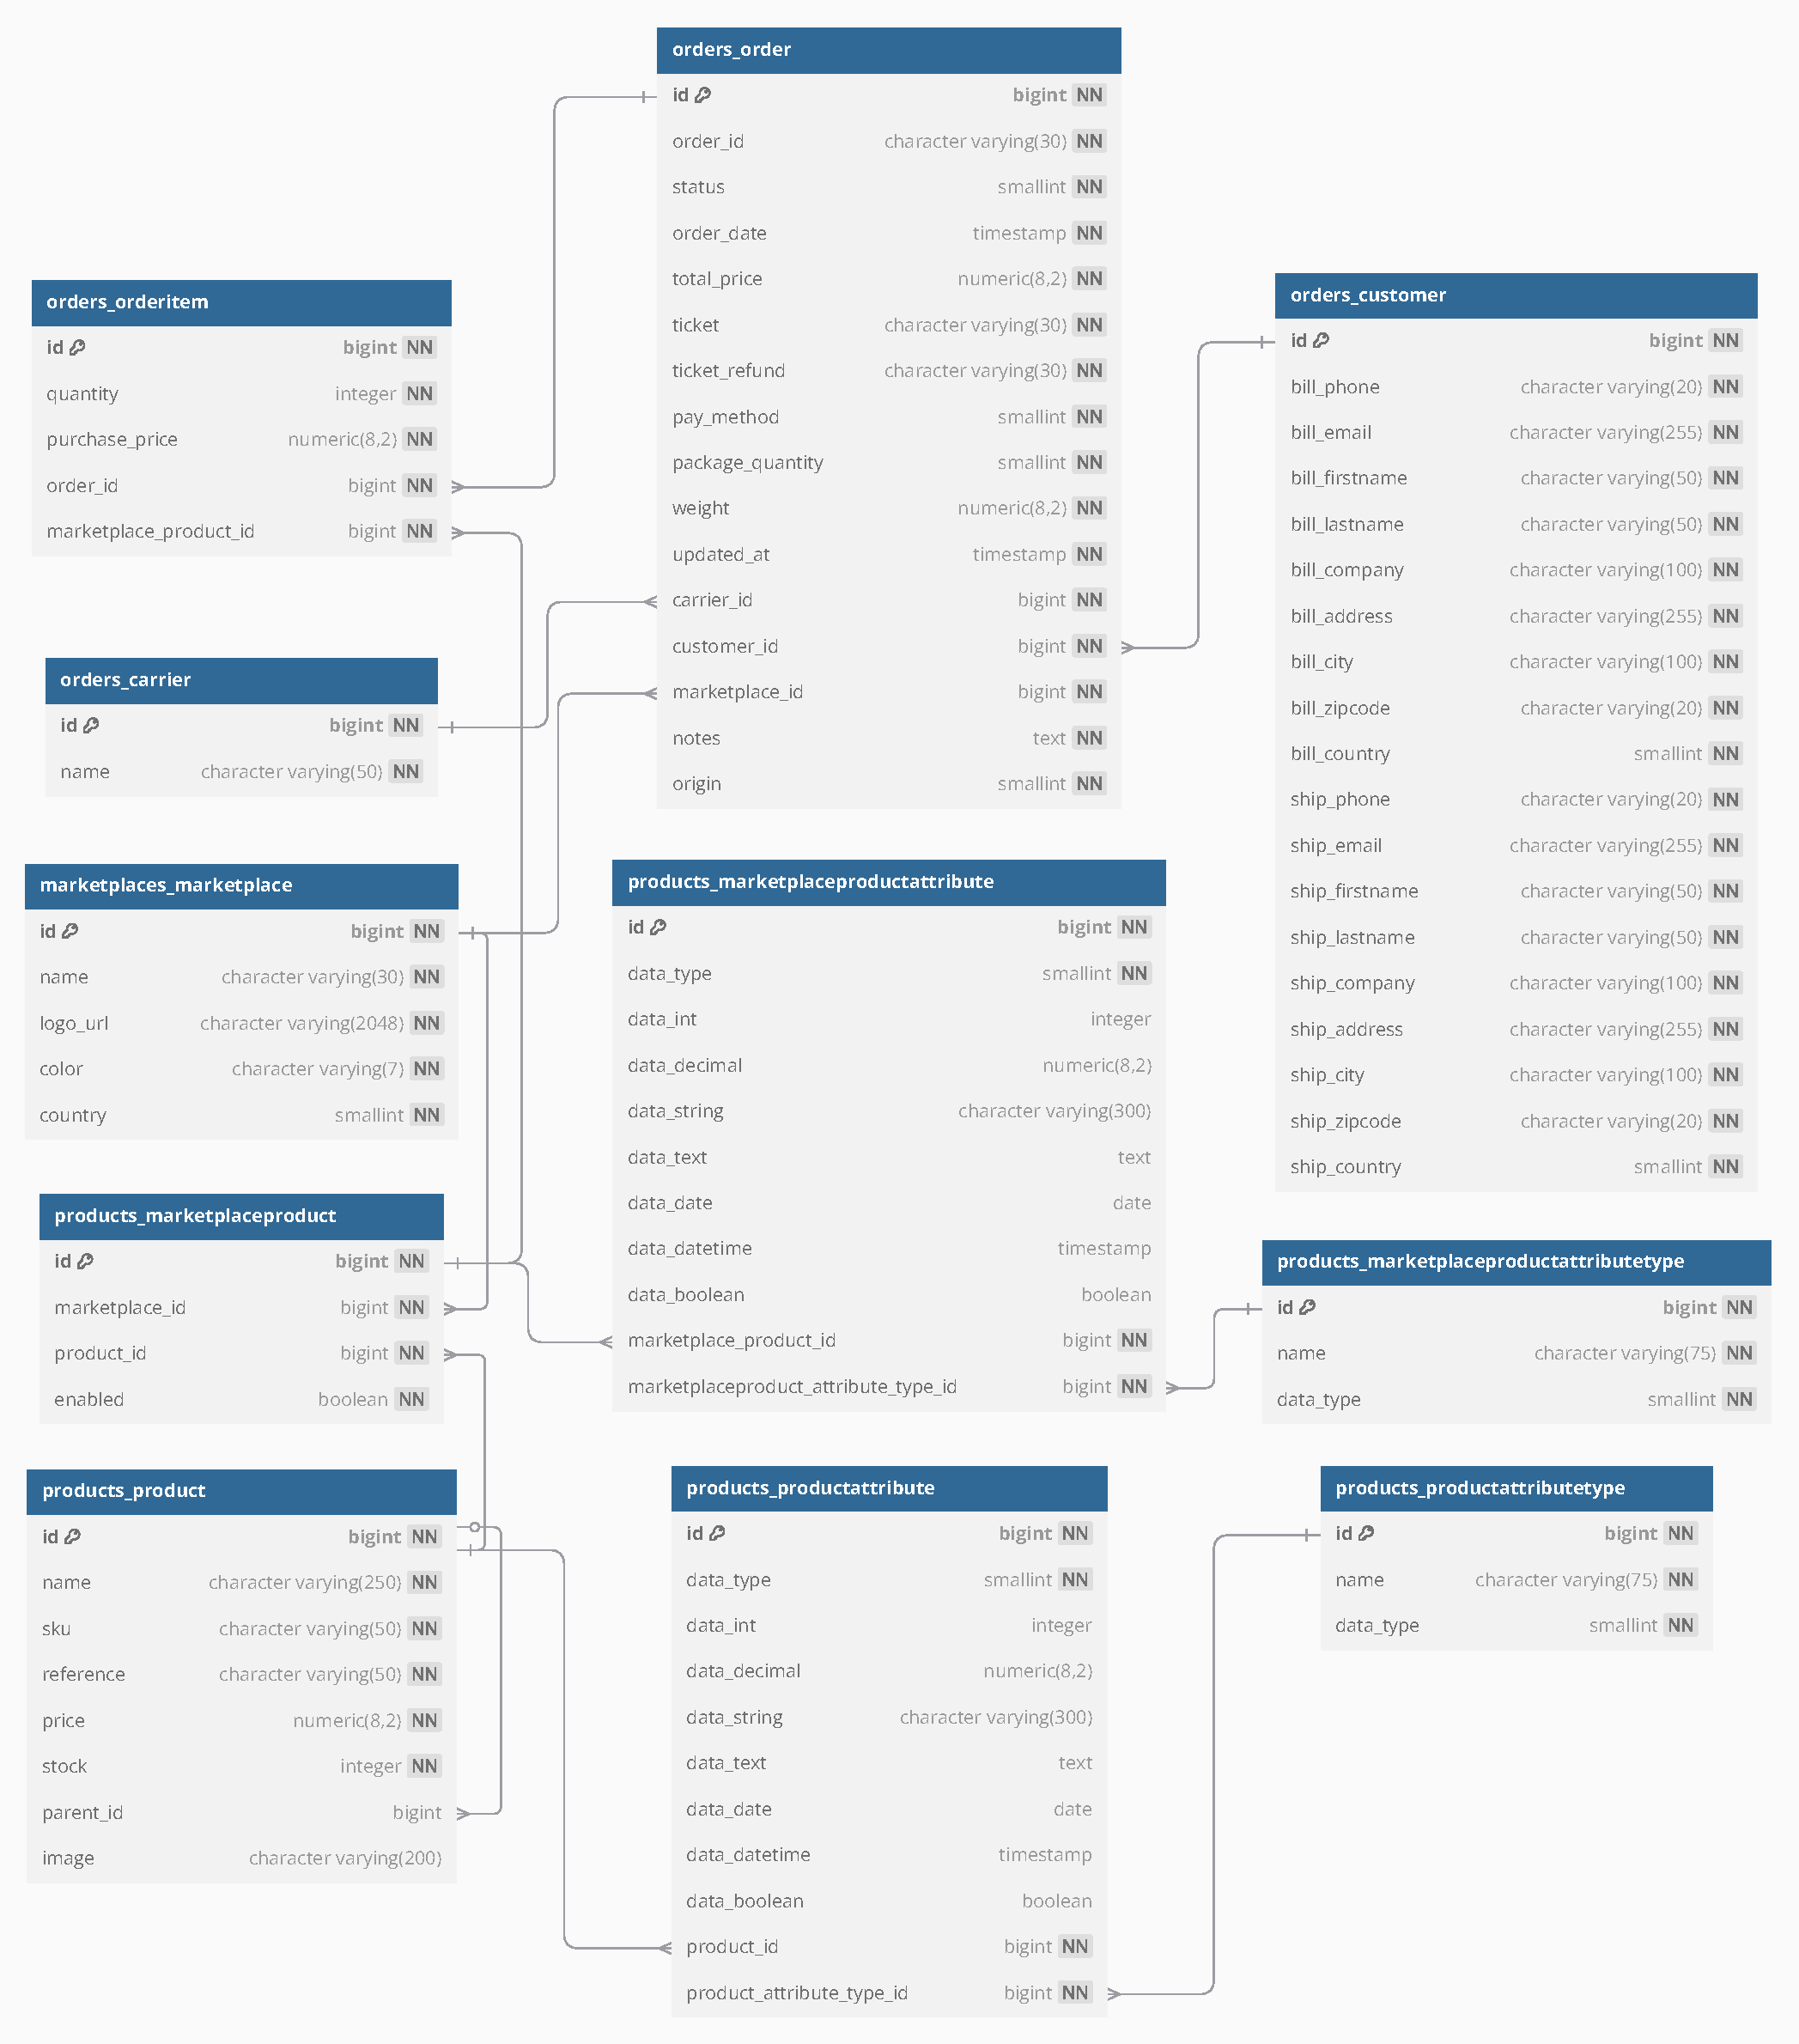
\includegraphics[width=0.98\textwidth]{figures/design_develop/database_diagram.pdf}
    \caption{Diagrama de la base de datos}
    \label{fig:diagrama_base_datos}
\end{figure}

\section{Desarrollo del \textit{backend}}


\section{Desarrollo del \textit{frontend}}